%%%%%%%%%%%%%%%%%%%%%%%%%%%%%%%%%%%%%%%%%%%%%%%%%%%%%%%%%%%%%%%%%%%%%%%%%%%%%%%%%%
%%																				%%
%% File name: 		20hannes.tex												%%
%% Project name:	Hochleistungsantenne										%%
%% Type of work:	T3X00 project work											%%
%% Author:			Sarah Brückner, Maximilian Stiefel, Hannes Bohnengel		%%
%% Date:			10th July 2016												%%
%% University:		DHBW Ravensburg Campus Friedrichshafen						%%
%% Comments:		Created in gedit with tab width = 4							%%
%%																				%%
%%%%%%%%%%%%%%%%%%%%%%%%%%%%%%%%%%%%%%%%%%%%%%%%%%%%%%%%%%%%%%%%%%%%%%%%%%%%%%%%%%

\chapter{GPredict}

Eine sehr detaillierte Beschreibung der Software GPredict ist unter \cite{gpredictmanual} in englischer Sprache verfügbar. Dieses Kapitel stellt eine kompakte Beschreibung mit ausschließlich für dieses Projekt relevanten Informationen dar. Insofern können gewisse Parallelen nicht ausgeschlossen werden, wobei darauf hingewiesen sei, dass der Mehrwert dieser Zusammenfassung in der Kürze und Relevanz im Vergleich zum englischen Pendant liegt.

\section{Übersicht}

GPredict ist eine freie Software zur Satellitenverfolgung und Orbitvorhersage und steht als Quellcode oder bereits fertig kompiliertes Programm für Windows, Mac OS und Linux zur Verfügung. Die Software ist in C geschrieben und unter der GNU \ac{GPL} lizenziert, somit kann sie frei verändert und an die entsprechenden Nutzervoraussetzungen angepasst werden. Im Rahmen dieser Projektarbeit wird Version 1.3 von GPredict verwendet (verfügbar unter \cite{gpredictdownload}).\newpar
In Abbildung \ref{fig:gpredict-principle} ist das Prinzip eines Satellitenverfolgungsprogramms zu sehen (die blauen Blöcke stellen hierbei die Funktionalität des Programms dar). Zunächst wird an Hand der Keplerschen Bahnelemente und dem aktuellen Zeitpunkt die absolute Position des Satelliten berechnet. Daraufhin wird der Vektor, der von der Bodenstation zum Satelliten zeigt, bestimmt. Nun können Azimut und Elevation dieses Vektors für die Ansteuerung der Antenne verwendet werden.

\begin{figure}[h]
	\centering
	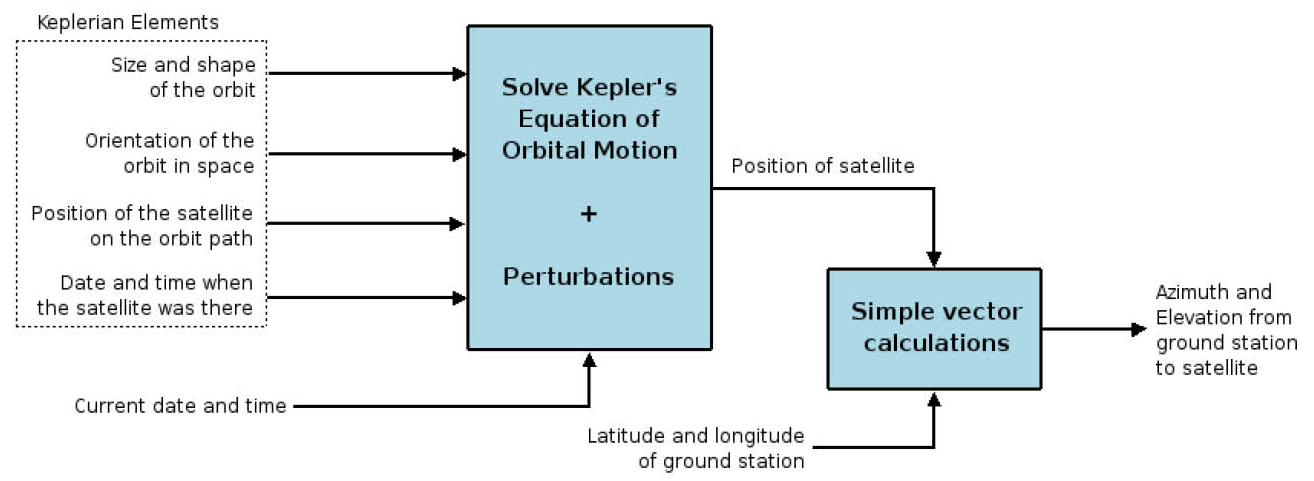
\includegraphics[width=1\textwidth]{gpredict-principle}
	\caption{Prinzip eines Satellitenverfolgungsprogramms, Quelle: \cite{gpredictmanual}}
	\label{fig:gpredict-principle} 
\end{figure}

\clearpage

% \label{chap:models} für XXX
Zur Berechnung der Satellitenposition wird auf den NORAD SGP4/SDP4 Algorithmus zurückgegriffen (siehe Abschnitt XXX). Um hierfür zu jedem Zeitpunkt die aktuellen Kepler-Elemente des zu verfolgenden Satelliten zu kennen, gibt es unter GPredict die Möglichkeit einer automatischen Aktualisierung über HTTP, FTP oder aus dem lokalen Verzeichnis.\newpar
Bei GPredict ist im Gegensatz zu anderen Satellitenverfolgungsprogrammen wie SatPC32 kein Limit an zu verfolgenden Satelliten und Bodenstationen gegeben. Durch die Verwendung von Modulen kann außerdem unkompliziert zwischen verschiedenen Konfigurationen gewechselt werden. Die Orbitvorhersage eines Satelliten lässt sich sowohl grafisch als auch tabellarisch darstellen, wobei durch die Einstellungen verschiedenster Parameter eine sehr individuelle Anzeige erreicht werden kann.

\section{Grafische Oberfläche}

In Abbildung \ref{fig:gpredictstartup} ist die grafische Oberfläche von GPredict zu sehen. In der Standardkonfiguration ist dort zunächst die Kartenansicht bzw. \myemph{Map View} (oben), die Polaransicht bwz. \myemph{Polar View} (links unten) und die Einzelsatellitenansicht bzw. \myemph{Single-Satellite View} (rechts unten) zu sehen.

\begin{figure}[h]
	\centering
	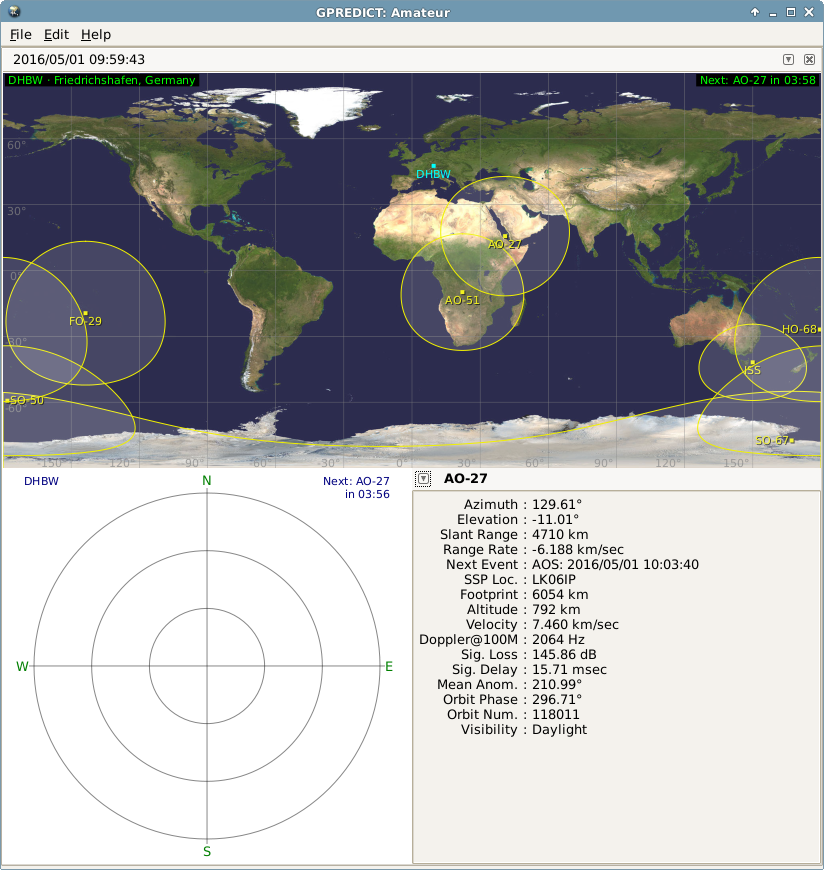
\includegraphics[width=0.54\textwidth]{gpredict-startup}
	\caption{Standardoberfläche von GPredict}
	\label{fig:gpredictstartup} 
\end{figure}

\clearpage

\subsection{Grundansichten}

Zu den oben genannten Ansichten kommen noch zwei Weitere hinzu, die Listenansicht bzw. \myemph{List View} und eine Ansicht für bevorstehende Durchläufe, die sogenannte \myemph{Upcoming Passes View}. Im Folgenden werden die verschiedenen Ansichten genauer beschrieben:\newpar
\textbf{Map View}\\
Diese Ansicht besteht, wie in Abbildung \ref{fig:gpredictstartup} zu sehen, aus einer Weltkarte auf der die aktuellen Standorte der für das aktuelle Modul ausgewählten Satelliten zu sehen ist. Das heißt der Punkt auf dem der entsprechende Satellit senkrecht bezogen auf den Erdmittelpunkt steht. Außerdem ist um diesen Punkt die Fläche umrahmt, von der der Satellit von der Erde aus sichtbar ist. Mit einem Rechtsklick auf einen Satellitennamen kann außerdem die Option \myemph{Ground Track} aktiviert werden, mit welcher die Spur des Satelliten für mehrere Orbits angezeigt wird.\newpar
\textbf{Polar View}\\
Die \myemph{Polar View} (siehe Abbildung \ref{fig:gpredictstartup}) stellt eine Draufsicht auf die Bodenstation dar, bei der die Polarachse den Azimutwinkel darstellt und die Radialachse den Elevationswinkel. Mit einem Rechtsklick auf einen Satelliten lässt sich mit der Option \myemph{Show sky track} aktivieren, das die Spur des entsprechenden Satelliten anzeigt wird. Zusätzlich wird das aktuelle Modul links oben angezeigt, der nächste sichtbare Satellit (rechts oben) und die genauen Werte für Azimut und Elevation (links unten) sobald sich der Mauszeiger auf der \myemph{Polar View} befindet.\newpar
\textbf{Single-Satellite View}\\
In dieser Ansicht (siehe Abbildung \ref{fig:gpredictstartup}) werden detaillierte Informationen zu einem ausgewählten Satelliten angezeigt, z.B. Azimut, Elevation, Entfernung der direkten Sichtverbindung (\myemph{Slant Range}), Höhe, Geschwindigkeit, Doppler-Verschiebung oder Signaldämpfung. Mit einem Klick auf das \myvsymbol-Symbol links neben dem Satellitennamen kann zwischen den für dieses Modul ausgewählten Satelliten gewechselt werden.

\clearpage

\textbf{List View}\\
Die Listenansicht zeigt eine tabellarische Auflistung aller für das aktuelle Modul ausgewählten Satelliten mit verschiedenen Details, mit je einem Satelliten pro Zeile. In Abbildung \ref{fig:listview} ist die Listenansicht mit allen verfügbaren Details zu sehen. Mit einem Klick auf eine entsprechende Kategorie lässt sich das Sortierkriterium ändern. Falls hier ein variables Kriterium wie die Geschwindigkeit eingestellt wird, ändert sich die Sortierreihenfolge mit der eingestellten Auffrischrate (\myemph{Refresh Rate}). Die Bezeichnung des jeweiligen Details ist in dieser Ansicht abgekürzt, z.B. \myemph{Az} für \myemph{Azimut}. Unter den Moduleinstellungen beim Reiter \myemph{List View} kann ausgewählt werden, welches Detail angezeigt wird. Dort ist außerdem erkenntlich für was die entsprechenden Abkürzungen stehen.

\begin{figure}[h]
	\centering
	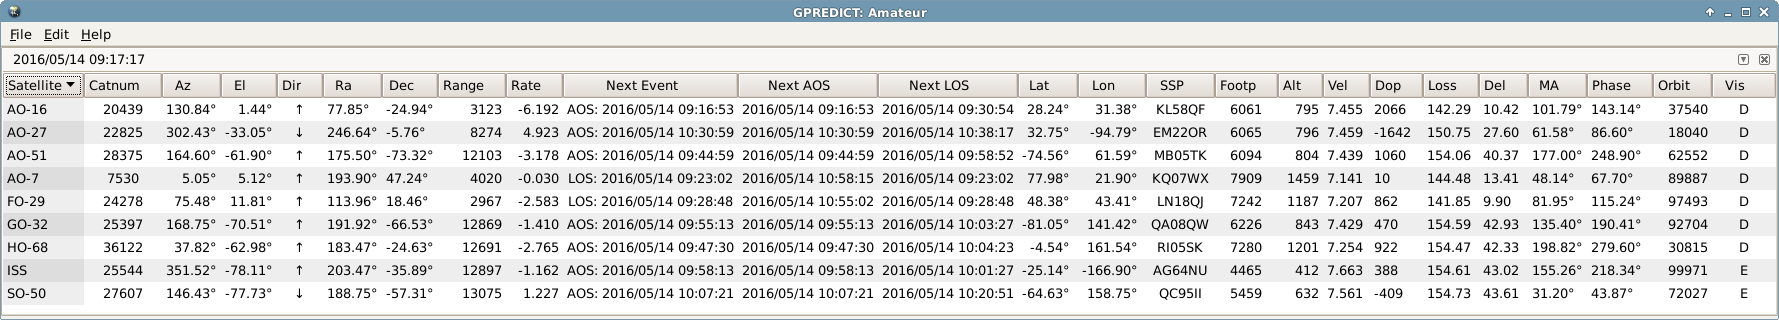
\includegraphics[width=1\textwidth]{listview}
	\caption{\myemph{List View}}
	\label{fig:listview} 
\end{figure}

\textbf{Upcoming Passes View}\\
Die \myemph{Upcoming Passes View} (siehe Abbildung \ref{fig:upcomingpassesview}) zeigt alle Satelliten des aktuellen Moduls, deren Azimut und Elevation, sowie die Zeit bis zum nächsten Verschwinden des Satelliten, dem sogenannten \myemph{\ac{LOS}} bzw. dem nächsten Auftauchen, auch \myemph{\ac{AOS}} genannt. Wie bei der \myemph{List View} ist es auch hier möglich nach den verschiedenen Spalten zu sortieren.

\begin{figure}[h]
	\centering
	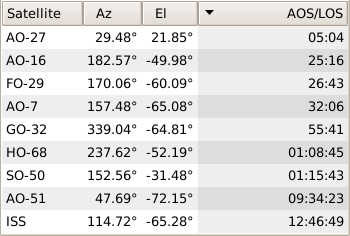
\includegraphics[width=0.4\textwidth]{upcomingpassesview}
	\caption{\myemph{Upcoming Passes View}}
	\label{fig:upcomingpassesview} 
\end{figure}

\clearpage

\subsection{Weitere Ansichten}

Bei allen Ansichten kann durch einen Klick auf den Satellitennamen ein kleines Pop-Up Menü geöffnet werden, welches den entsprechenden Satellitennamen, die Option \myemph{Show next pass} und die Option \myemph{Future passes} anzeigt. Bei einem Klick auf den Satellitennamen öffnet sich ein Fenster mit dem Titel \myemph{Satellite Info}, wie in Abbildung \ref{fig:satinfo} zu sehen. Dort sind unter dem Reiter \myemph{Orbit Info} verschiedene Informationen zum Satellitenorbit und unter dem Reiter \myemph{Transponders} die verfügbaren Transponder zu sehen.

% (bei der \myemph{Single-Satellite View} ein Klick auf das Dreieck neben dem Namen)
% (oder einen Doppelklick in der entsprechenden Ansicht auf den Satellitennamen)

\begin{figure}[h]
	\centering
	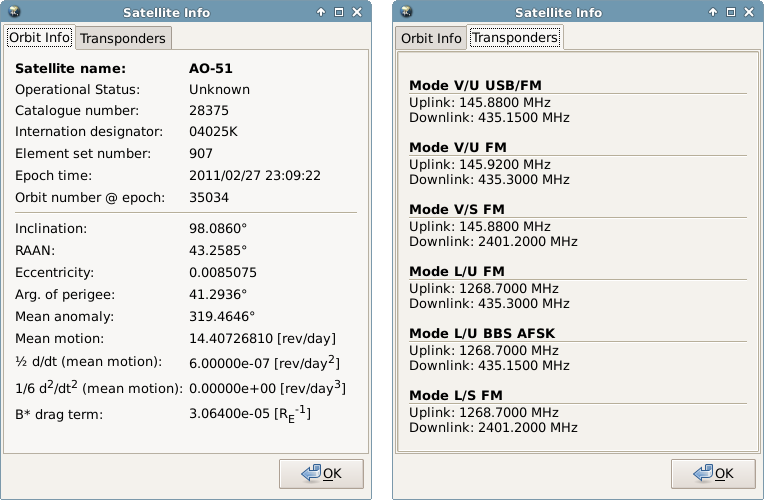
\includegraphics[width=0.65\textwidth]{satinfo}
	\caption{\myemph{Satellite Info}}
	\label{fig:satinfo} 
\end{figure}

Mit einem Klick auf die Option \myemph{Show next pass} gelangt man zu einer Übersicht über den nächsten Durchlauf des entsprechenden Satelliten. Die Details sind tabellarisch, als Polaransicht und als Verlauf des Azimut- und Elevationswinkels über der Zeit zu sehen (siehe Abbildung \ref{fig:passdetails}).

\begin{figure}[h]
	\centering
	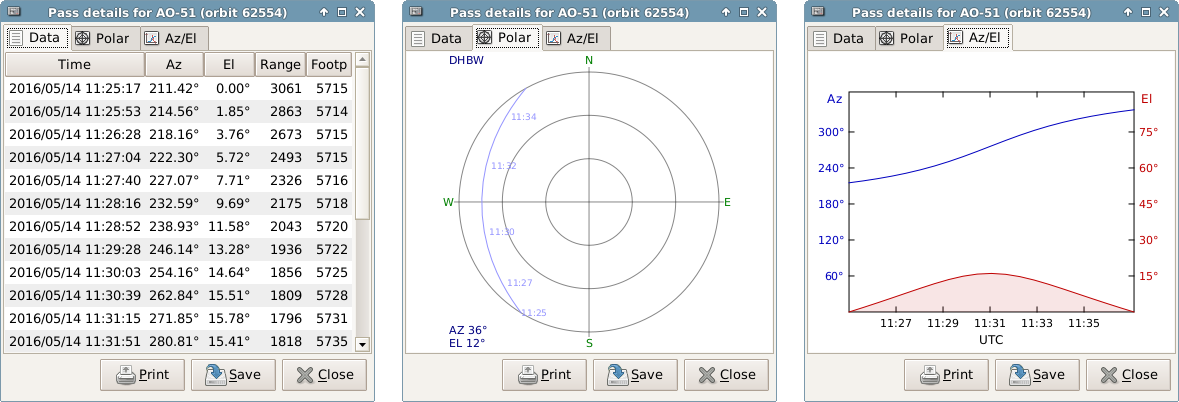
\includegraphics[width=1\textwidth]{passdetails}
	\caption{\myemph{Pass Details}}
	\label{fig:passdetails} 
\end{figure}

\clearpage

Die Option \myemph{Future passes} öffnet ein Fenster, in welchem die nächsten Durchläufe des entsprechenden Satelliten tabellarisch dargestellt sind (siehe Abbildung \ref{fig:upcomingpasses}). Hierbei ist die Anzahl der darzustellenden Durchläufe in den GPredict-Einstellungen unter \myemph{Predict} als \myemph{Number of passes to predict} einstellbar.

\begin{figure}[h]
	\centering
	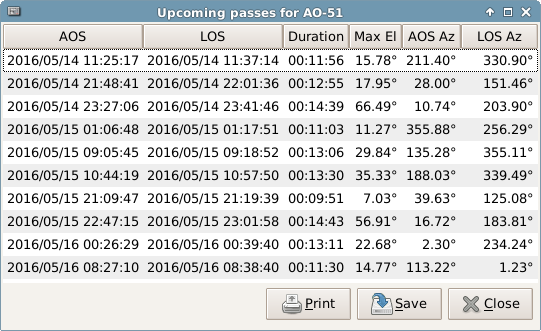
\includegraphics[width=0.5\textwidth]{upcomingpasses}
	\caption{\myemph{Upcoming Passes}}
	\label{fig:upcomingpasses} 
\end{figure}

\vspace{-0.5em}

\subsection{Modul Pop-Up Menü}

Um das Modul Pop-Up Menü zu öffnen, klickt man ganz rechts oben im GPredict-Fenster auf das \myvsymbol-Symbol. Im daraufhin erscheinenden Pop-Up Menü ist es möglich die Positionierung eines Moduls innerhalb des GPredict-Fensters einzustellen, ein Modul zu kopieren, zu löschen, zu schließen oder genauer zu konfigurieren. Außerdem sind dort weitere Funktionen, welche im Folgenden genauer beschrieben werden, zugänglich.\newpar
Wie in Abbildung \ref{fig:theskyataglance} zu sehen, bietet die Funktion \myemph{Sky at a glance} eine Übersicht darüber, wann welche Satelliten innerhalb der nächsten acht Stunden sichtbar sind. Dieser Zeitraum lässt sich in den GPredict-Einstellungen bei \myemph{Predict} unter dem Reiter \myemph{Sky at a Glance} zwischen einer und 24 Stunden einstellen.

\begin{figure}[h]
	\centering
	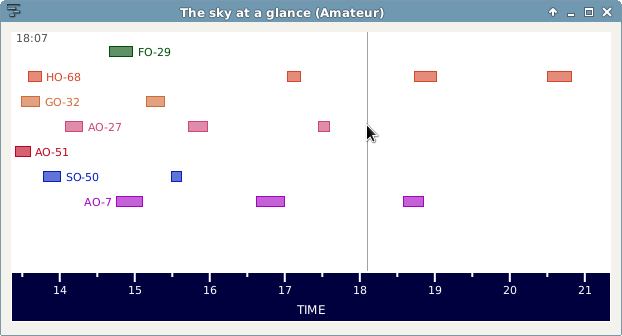
\includegraphics[width=0.5\textwidth]{theskyataglance}
	\caption{\myemph{The sky at a glance}}
	\label{fig:theskyataglance} 
\end{figure}

\clearpage

Über die Funktion \myemph{Time Controller} (siehe Abbildung \ref{fig:timecontroller}) lässt sich die Zeit, auf die sich die Berechnungen von GPredict beziehen, ändern. Hierbei ist standardmäßig das aktuelle Datum und die aktuelle Uhrzeit eingestellt. Außerdem kann hier die Geschwindigkeit, mit der die eingestellte Zeit fortschreitet, auf maximal ein Hundertfaches erhöht werden. Die eingestellte Zeit wird im GPredict-Fenster ganz links oben im ausgewählten Format angezeigt. Mit dem Schieberegler kann die Zeit zwischen --2,5 und +2,5 Stunden eingestellt werden.

\begin{figure}[h]
	\centering
	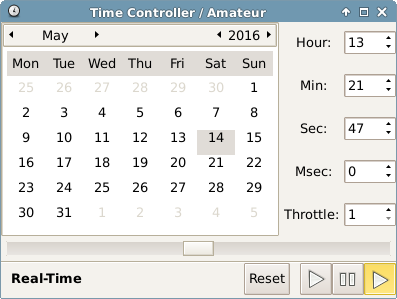
\includegraphics[width=0.35\textwidth]{timecontroller}
	\caption{\myemph{Time Controller}}
	\label{fig:timecontroller} 
\end{figure}

Klickt man auf \myemph{Configure}, öffnet sich ein Fenster wie in Abbildung \ref{fig:editmodule} zu sehen. Hier lassen sich die zu verfolgenden Satelliten und die Bodenstation für das aktuelle Modul auswählen. Außerdem gelangt man mit einem Klick auf das Feld \myemph{Properties} in die Modul-Einstellungen. Diese gelten im Gegensatz zu den in den allgemeinen GPredict-Einstellungen zu findenden Modul-Einstellungen nur für das aktuelle Modul. Auf Seite \pageref{modulesettingsgeneral} sind nähere Infos zu den Modul-Einstellungen zu finden.
\label{modulesettingsspecific}

\begin{figure}[h]
	\centering
	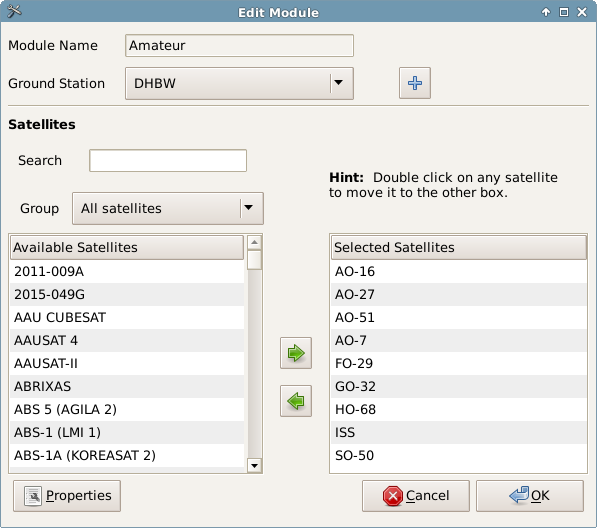
\includegraphics[width=0.5\textwidth]{editmodule}
	\caption{\myemph{Edit Module}}
	\label{fig:editmodule} 
\end{figure}

\clearpage

Hinter der Funktion \myemph{Antenna Control} (siehe Abbildung \ref{fig:rotatorcontrol}) verbirgt sich ein Bedienfeld zur Steuerung der Antennenrotoren. Bevor dieses geöffnet werden kann, muss zunächst in den GPredict-Einstellungen unter \myemph{Interfaces} mindestens eine Schnittstelle zur Rotorensteuerung konfiguriert werden (siehe Abschnitt XXX). 
\begin{figure}[h]
	\centering
	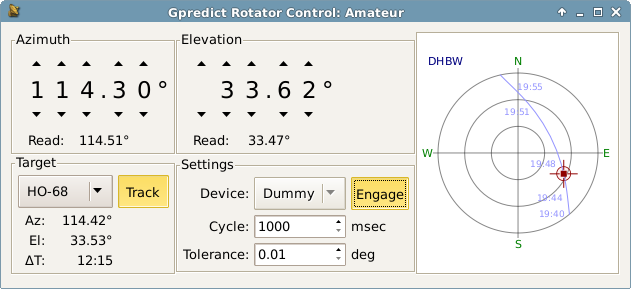
\includegraphics[width=0.6\textwidth]{rotatorcontrol-active}
	\caption{Rotorensteuerungs-Bedienfeld}
	\label{fig:rotatorcontrol} 
\end{figure}

Das Bedienfeld beinhaltet zum Einen eine Polaransicht, auf der die Spur und der aktuelle Ort des zu verfolgenden Satelliten (dargestellt durch ein Viereck) und die gegenwärtige Ausrichtung der Antenne (dargestellt durch ein Fadenkreuz) zu sehen ist. Zum Anderen sind folgende vier Bereiche verfügbar:

\begin{itemize}
	\parskip0pt
	\item \textbf{Azimuth:} In diesem Feld lässt sich die Ausrichtung der Antenne in Azimut-Richtung steuern, vorausgesetzt, dass die \myemph{Track}-Funktion nicht aktiviert ist. Am unteren Ende des Feldes wird unter \myemph{Read} der aktuelle Azimut-Winkel der Antenne angezeigt. Ist keine Verbindung zum Rotor aufgebaut, wird hier ,,-\,-\,-'' angezeigt. Liegt ein Verbindungsproblem vor, erscheint ,,ERROR''.
	\item \textbf{Elevation:} In diesem Feld lässt sich die Ausrichtung der Antenne in Elevations-Richtung steuern, vorausgesetzt, dass die \myemph{Track}-Funktion nicht aktiviert ist. Am unteren Ende des Feldes wird unter \myemph{Read} der aktuelle Elevations-Winkel der Antenne angezeigt. Ist keine Verbindung zum Rotor aufgebaut, wird hier ,,-\,-\,-'' angezeigt. Liegt ein Verbindungsproblem vor, erscheint ,,ERROR''.
	\item \textbf{Target:} Hier lässt sich der zu verfolgende Satellit auswählen. Es stehen hierbei nur die für das aktuelle Modul ausgewählten Satelliten zu Verfügung. Aktiviert man die Schaltfläche \myemph{Track}, wird der ausgewählte Satellit verfolgt. Unter dem Satellitennamen werden die jeweiligen Winkel in Echtzeit dargestellt und hinter $\Delta$T wird die Zeit bis zum nächsten \ac{AOS} bzw. \ac{LOS} angezeigt.
	\clearpage
	\item \textbf{Settings:} Hier lässt sich die in den GPredict-Einstellungen festgelegte Schnittstelle zur Kommunikation mit den Rotoren auswählen. Mit einem Klick auf die Schaltfläche \myemph{Engage} wird die Verbindung zu dieser Schnittstelle aufgebaut bzw. unterbrochen. Unter \myemph{Cycle} kann dabei der Zyklus eingestellt werden, in welchem Kommandos an die Rotor-Schnittstelle gesendet und Winkelwerte von dieser abgefragt werden. Ein sinnvoller Wert liegt hierbei zwischen zwei und fünf Sekunden. Bei \myemph{Tolerance} wird die tolerierte Differenz zwischen abgefragtem und eingestelltem Winkel eingetragen. Sobald diese überschritten wird, wird ein  Kommando an die Rotor-Schnittstelle geschickt. Hierbei sollte sowohl die Winkelauflösung der Rotorensteuerung, als auch die Keulenbreite der Antenne berücksichtigt werden. Nach fünf aufeinanderfolgenden Fehlern bei der Kommunikation mit den Rotoren, wird die Verbindung automatisch unterbrochen.
\end{itemize}

In Tabelle \ref{tab:rotatorcontrolmodes} sind alle möglichen Kombinationen der Schaltflächen \myemph{Track} und \myemph{Engage} und deren Auswirkung beschrieben.

\begin{table}[h]
	\begin{tabularx}{\textwidth}{|l|l|X|}
		\hline
		\textbf{Track} 	    & \textbf{Engage}	&\textbf{Beschreibung}\\
		\hline
		Inaktiv          	& Inaktiv 			& Es werden weder Kommandos an die Rotoren gesendet, noch wird die aktuelle Ausrichtung der Antenne ausgelesen. Die aktuellen Winkel des zu verfolgenden Satelliten werden nicht in die Winkelsteuerungs-Eingabefelder übertragen.\\
		Aktiv              	& Inaktiv   		& Die aktuellen Winkel des zu verfolgenden Satelliten werden in die Winkelsteuerungs-Eingabefelder übertragen, es werden aber keine Kommandos an die Rotoren geschickt und die aktuelle Ausrichtung der Antenne wird nicht ausgelesen.\\
		Aktiv              	& Aktiv	            & Die aktuellen Winkel des zu verfolgenden Satelliten werden in die Winkelsteuerungs-Eingabefelder übertragen und diese werden an die Rotoren geschickt. Die aktuelle Ausrichtung der Antenne wird ausgelesen.\\
		Inaktiv            	& Aktiv   			& Die Winkel, die in den Winkelsteuerungs-Eingabefelder eingestellt sind, werden an die Rotoren gesendet und die aktuelle Ausrichtung der Antenne wird ausgelesen.\\
		\hline		
	\end{tabularx}
	\caption{Betriebsmodi des \myemph{Antenna Control}-Bedienfelds, Quelle: \cite{gpredictmanual} \vspace{-2em}}
	\label{tab:rotatorcontrolmodes}
\end{table}

\newpage

Um dem Funkgerät die entsprechenden Up- und Downlink-Frequenzen inklusive Korrektur der Doppler-Verschiebung zu übermitteln, wird das \myemph{Radio Control}-Bedienfeld (siehe Abbildung \ref{fig:radiocontrol}) verwendet. Dieses kann nur geöffnet werden, wenn mindestens eine Funkgerät-Schnittstelle in den GPredict-Einstellungen unter \myemph{Interfaces} konfiguriert ist (siehe Abschnitt XXX).

\begin{figure}[h]
	\centering
	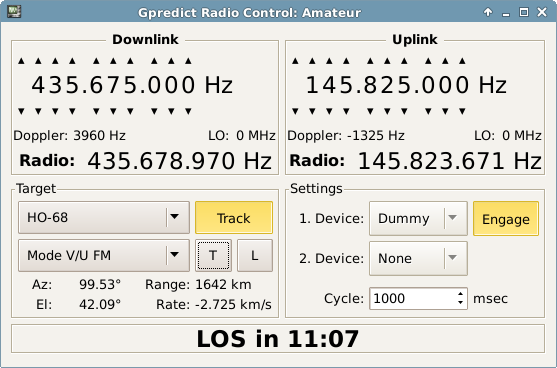
\includegraphics[width=0.6\textwidth]{radiocontrol-active}
	\caption{Funkgerät-Steuerung}
	\label{fig:radiocontrol} 
\end{figure}

Neben einer Anzeige die die Zeit bis zum nächsten \ac{AOS} bzw. \ac{LOS} darstellt (ganz unten im Bedienfeld in fettgedruckten Buchstaben) kann das \myemph{Radio Control}-Bedienfeld in folgende vier Bereiche untergliedert werden:

\begin{itemize}
	\parskip0pt
	\item \textbf{Downlink:} In diesem Bereich kann die Frequenzeinstellung für die Downlink-Frequenz vorgenommen werden. Außerdem ist die aktuelle Dopplerfrequenz und ein Feld names \myemph{LO}, welches für eine Offsetfrequenz steht, die im Funkgerät eingestellt werden kann, steht. Die korrigierte Frequenz welche nach \myemph{Radio} angezeigt wird, setzt sich damit beispielsweise wie folgt zusammen: $f_{Radio} = f_{Satellite} + f_{Doppler} - f_{LO}$
	\item \textbf{Uplink:} Dieser Bereich beinhaltet die Frequenzeinstellungen für die Uplink-Frequenz und besitzt die gleichen Eigenschaften wie der Downlink-Bereich.
	\item \textbf{Target:} Hier kann der zu verfolgende Satellit und der zu verwendente Transponder eingestellt werden. Mit einem Klick auf \myemph{Track} wird die Doppler-Verschiebung des ausgewählten Satelliten bei den Frequenzeinstellungen im Downlink- und Uplink-Bereich korrigiert. Eine wichtige Rolle spielt hierbei die Schaltfläche \myemph{T} (\myemph{Tune}), da die Frequenzen des Transponders nur durch einen Klick auf diese in die Frequenzeinstellungen übertragen werden. Sollte der Transponder beispielsweise nur einen Downlink besitzen, wird auch nur die Frequenz im Downlink-Bereich eingestellt.
	Mit der Schaltfläche \myemph{L} (\myemph{Lock}) lässt sich die Differenz der Downlink- und Uplink-Frequenz sperren, das heißt Änderungen an der einen wirken sich auch auf die andere Frequenz aus. Dies ist nicht für Transponder möglich, die nur einen Up- oder Downlink besitzen.
	\item \textbf{Settings:} In diesem Bereich lassen sich bis zu zwei Funkgeräte auswählen die in den GPredict-Einstellungen unter \myemph{Interfaces} eingerichtet wurden. Das obere Gerät stellt das Primäre dar und kann für Up- und Downlink verwendet werden. Das Untere kann als sekundäres Gerät verwendet werden, welches nur für den Uplink verwendet werden kann. Mit einem Klick auf \myemph{Engage} wird die Kommunikation zwischen GPredict und Funkgerät(en) aufgebaut. Hierbei kann im Feld neben \myemph{Cycle} der Zyklus eingetragen werden, nach welchem Kommandos an das Funkgerät geschickt werden sollen.
\end{itemize}

In Tabelle \ref{tab:radiocontrolmodes} ist eine Übersicht über die verschiedenen Betriebsmodi des \myemph{Radio Control}-Bedienfelds zu sehen.

\begin{table}[h]
	\begin{tabularx}{\textwidth}{|l|l|X|}
		\hline
		\textbf{Track} 	    & \textbf{Engage}	&\textbf{Beschreibung}\\
		\hline
		Inaktiv          	& Inaktiv 			& Es wird keine Korrektur der Doppler-Verschiebung durchgeführt, keine Befehle an das Funkgerät gesendet und die aktuelle Frequenz des Funkgeräts nicht ausgelesen.\\
		Aktiv              	& Inaktiv   		& Die Korrektur der Doppler-Verschiebung wird durchgeführt, es werden aber weder Befehle an das Funkgerät geschickt noch wird die aktuelle Frequenz ausgelesen.\\
		Aktiv              	& Aktiv	            & Die Doppler-Verschiebung wird korrigiert und die eingestellte Frequenz wird zum Funkgerät geschickt. Die aktuelle Frequenz des Funkgeräts wird ausgelesen.\\
		Inaktiv            	& Aktiv   			& Die Korrektur der Doppler-Verschiebung wird nicht ausgeführt. Die eingestellte Frequenz wird an das Funkgerät geschickt und die dort eingestellte Frequenz wird ausgelesen.\\
		\hline		
	\end{tabularx}
	\caption{Betriebsmodi des \myemph{Radio Control}-Bedienfelds, Quelle: \cite{gpredictmanual}}
	\label{tab:radiocontrolmodes}
\end{table}

\newpage

Wenn die \myemph{Engage}-Schaltfläche aktiviert ist, wird die Korrektur der Doppler-Verschiebung durchgeführt, egal ob der ausgewählte Satellit sichtbar ist oder nicht.

\subsection{GPredict-Einstellungen}

Um in die GPredict-Einstellungen zu gelangen, klickt man links oben unterhalb der Titelleiste auf \myemph{Edit} und anschließend auf \myemph{Preferences}. Nun öffnet sich ein Fenster bei dem standardmäßig die Erste der vier Kategorien zu sehen ist, die Kategorie \myemph{General} (siehe Abbildung \ref{fig:generalsettings}). Nach einer Veränderung in den GPredict-Einstellungen muss GPredict zunächst neugestartet werden, damit diese Änderung wirksam wird. Überall wo die Schaltfläche \myemph{Reset} zu finden ist, können mit einem Klick auf diese, die Standard-Einstellungen wiederhergestellt werden. Bei den meisten Optionen erscheint ein kleines Informations-Fenster, sobald man mit dem Mauszeiger einige Sekunden über der entsprechenden Option verharrt.

\begin{figure}[h]
	\centering
	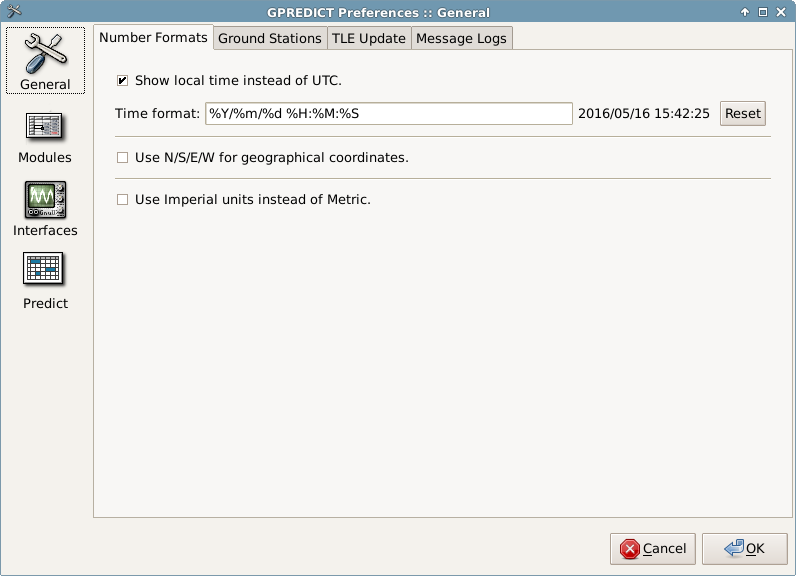
\includegraphics[width=0.65\textwidth]{generalsettings}
	\caption{GPredict-Einstellungen, Kategorie \myemph{General}}
	\label{fig:generalsettings} 
\end{figure}

Die Kategorie \myemph{General} ist in folgende vier Reiter untergliedert:

\begin{itemize}
	\parskip0pt
	\item \textbf{Number Formats:} Hier lassen sich Einstellungen zum Zeitformat, zu den geografischen Koordinaten und zu den Längen- und Geschwindigkeits-Einheiten vornehmen.
	\item \textbf{Ground Stations:} Unter diesem Reiter können beliebig viele Bodenstationen eingerichtet werden. Mindestens eine muss jedoch zu jeder Zeit vorhanden sein.
	\item \textbf{TLE Update:} Hier können Einstellungen zur Aktualisierung der Kepler-Elemente vorgenommen werden.
	\item \textbf{Message Logs:} Hier können Einstellungen bzgl. des GPredict-Protokolls vorgenommen werden. Unter \myemph{Log browser} im Menü \myemph{File} kann dieses dargestellt werden.
\end{itemize}

Zur Kategorie \myemph{Modules} gelangt man über zwei Wege. Der erste führt über die allgemeinen GPredict-Einstellungen, wie in diesem Abschnitt beschrieben. Der Zweite führt über das Modul Pop-Up Menü, wie auf Seite \pageref{modulesettingsspecific} beschrieben. Der Unterschied ist, dass bei den Modul-Einstellungen in den GPredict-Einstellungen die Standardwerte für alle Module eingestellt werden können und beim zweiten Weg nur die für das entsprechende Modul.
\label{modulesettingsgeneral}

%(siehe Abbildung \ref{fig:modulesettings})
\iffalse
\begin{figure}[h]
	\centering
	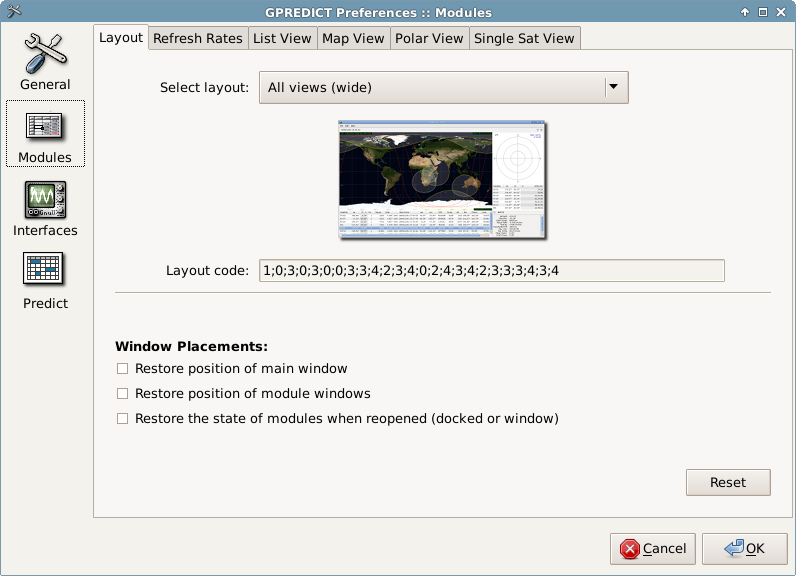
\includegraphics[width=0.65\textwidth]{modulesettings}
	\caption{GPredict-Einstellungen, Kategorie \myemph{Modules}}
	\label{fig:modulesettings} 
\end{figure}
\fi
Die Modul-Einstellungen sind in folgende sechs Reiter untergliedert:

\begin{itemize}
	\parskip0pt
	\item \textbf{Layout:} Bei diesem Reiter lässt sich konfigurieren, welche Ansichten in welcher Anordnung im GPredict-Fenster zu sehen sind. Hierbei kann aus verschiedenen Anordnungen ausgewählt werden oder eine völlig benutzerspezifische Anordnung erstellt werden (Hierfür wird an dieser Stelle auf \cite{gpredictmanual} Seite 67f verwiesen).
	\item \textbf{Refresh Rates:} Hier lässt sich die Zeitspanne auswählen, nach  welcher GPredict die Positions-Berechnungen periodisch für jeden Satelliten durchführt, der für das geöffnete Modul ausgewählt wurde. Außerdem lässt sich einstellen mit welchem ganzzahligem Vielfachen dieser Zeitspanne die einzelnen Ansichten aufgefrischt werden.
	\item \textbf{List View:} Hier lassen sich die Parameter der \myemph{List View} auswählen.
	\item \textbf{Map View:} Hier lassen sich Darstellungsoptionen für die \myemph{Map View} konfigurieren.
	\item \textbf{Polar View:} Hier lassen sich Darstellungsoptionen für die \myemph{Polar View} konfigurieren.
	\item \textbf{Single Sat View:} Hier lassen sich die Parameter der \myemph{Single Sat View} auswählen.
\end{itemize}

Die Kategorie \myemph{Interfaces} ist in zwei Reiter untergliedert, \myemph{Radios} und \myemph{Rotators}. Dort wird jeweils eine Liste der bereits eingerichteten Funkgeräte bzw. Rotoren angezeigt, welche standardmäßig leer ist. Die Anzahl der Geräte ist dabei nach oben nicht beschränkt. Die detaillierte Einrichtung ist in Abschnitt \ref{chap:radioconfig} und \ref{chap:rotatorconfig} genauer beschrieben.\newpar
Beim Öffnen der Kategorie \myemph{Predict} wird standardmäßig der Reiter \myemph{Pass Conditions} angezeigt. Unter diesem lassen sich folgende Parameter einstellen:

\begin{itemize}
	\parskip0pt
	\item \textbf{Minimum elevation:} Dieser Parameter gibt an, ab welcher Elevation von einem Durchlauf eines Satelliten ausgegangen wird. Das heißt, übersteigt die maximale Elevation diesen Wert, wird dieser Durchlauf in die \myemph{Upcoming Passes}, die \myemph{Pass Details} und die Ansicht \myemph{The sky at a glance} aufgenommen.
	\item \textbf{Number of passes to predict:} Anzahl der angezeigten zukünftigen Durchläufe.
	\item \textbf{Passes should occur within:} Dieser Parameter definiert den Zeitraum, in welchem zukünftige Durchläufe von GPredict berücksichtigt werden. So tritt entweder erst die Anzahl der angezeigten zukünftigen Durchläufe ein oder der Zeitraum in welchem zukünftige Durchläufe berücksichtigt werden sollen.
	\item \textbf{Time resolution:}	Hier kann die Zeitauflösung eingetragen werden, mit der der nächste Durchlauf in den \myemph{Pass Details} dargestellt wird. Je geringer die Auflösung, desto mehr Einträge werden angezeigt.
	\item \textbf{Number of entries:} Mit diesem Parameter kann die Anzahl der Eintrage des nächsten Durchlaufs in den \myemph{Pass Details} eingestellt werden. Hierbei ist zu beachten, dass diese Einstellung eine höhere Priorität als die Zeitauflösung besitzt.
	\item \textbf{Twilight threshold:} Dieser Parameter gibt an, ab welcher Elevation ein Satellit als sichtbar gilt. Für die Satellitenverfolgung spielt dieser Paramenter keine Rolle.
\end{itemize}

Unter den Reitern \myemph{Multiple Passes} und \myemph{Single Pass} lassen sich die Parameter auswählen, die in den Ansichten \myemph{Upcoming Passes} und \myemph{Pass Details} dargestellt werden, wohingegen beim Reiter \myemph{Sky at a Glance} Darstellungsoptionen für die Funktion \myemph{The sky at a glance} eingestellt werden können.\newpar
Eine detailliertere Beschreibung der GPredict-Einstellungen kann aus \cite{gpredictmanual} Seite 23ff entnommen werden.

\section{HamLib-Programmierschnittstelle}

\subsection{Übersicht}

Da es keinen einheitlichen Kommunikationsstandard für die zahlreichen Funkgeräte und Rotoren unterschiedlicher Hersteller gibt, ist für die Verwendung von GPredict eine applikationsspezifische Programmierschnittstelle oder auch \ac{API} erforderlich. Mit den \myemph{Ham Radio Control Libraries} (englisch für Amateurfunk-Kontrollbibliotheken), kurz HamLib, steht dem Benutzer eine solche \ac{API} zur Verfügung. HamLib ist unter der \ac{GPL} lizenziert und ist unter \cite{hamlibdownload} in der Version 3.0.1 als Download für Linux und Windows kostenlos verfügbar. Wie in Abbildung \ref{fig:hamlib} zu sehen, ermöglicht HamLib einer Software wie GPredict die Kommunikation mit verschiedenen Funkgeräten und Rotoren, in dem es für jedes dieser Geräte einen eigenen Treiber bzw. ein eigenes \ac{BE} zur Verfügung stellt.

\begin{figure}[h]
	\centering
	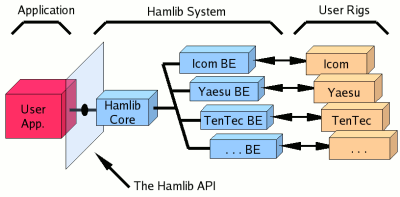
\includegraphics[width=0.5\textwidth]{hamlib}
	\caption{HamLib Design, Quelle: \cite{hamlibmanual}}
	\label{fig:hamlib} 
\end{figure}

Dabei verwendet man entweder den Quellcode um eine benutzerspezifische Anwendung zu erstellen oder man greift auf die bereits fertig kompilierten Programme zurück, welche im Folgenden aufgelistet sind:

\begin{itemize}
	\parskip0pt
	\item \textbf{rigctl:} Ein Kommandozeilenprogramm, mit welchem man Befehle über die Kommandozeile an das Funkgerät senden kann. (Unter Windows: \myemph{rigctl.exe})
	\item \textbf{rotctl:} Ein Kommandozeilenprogramm, mit welchem man Befehle über die Kommandozeile an die Antennenrotoren senden kann. (Unter Windows: \myemph{rotctl.exe})
	\item \textbf{rigctld:} Ein Kommandozeilenprogramm, mit welchem man Befehle über das TCP/IP-Protokoll an das Funkgerät senden kann (Unter Windows: \myemph{rigctld.exe})
	\item \textbf{rotctld:}  Ein Kommandozeilenprogramm, mit welchem man Befehle über das TCP/IP-Protokoll an die Antennenrotoren senden kann (Unter Windows: \myemph{rigctld.exe})
\end{itemize}

Hierbei steht ,,\myemph{rot}'' für ,,Rotator'' (deutsch: Rotor), ,,\myemph{rig}'' für  ,,Rig'' (deutsch: Amateurfunkgerät) und das ,,\myemph{d} am Ende von \myemph{rigctld} und \myemph{rotctld} für ,,Deamon'' (deutsch: Hintergrundprozess).

\subsection{Parameter-Konfiguration}
\label{chap:hamlibconfig}

Für die erfolgreiche Nutzung der oben genannten Programme müssen einige Optionen und Parameter berücksichtigt werden. Hierfür ist es notwendig die erforderlichen Informationen zu den Rotoren und zum Funkgerät zu kennen. Um eine Übersicht der möglichen Optionen und Befehle zu erhalten, kann das jeweilige Programm einfach mit der Option \texttt{-h} oder \texttt{-\,-help} ausgeführt werden (siehe Anhang XXX und YYY).\newpar
Die erste zentrale Information ist die \myemph{Hamlib ID}. Hierfür gibt man folgenden Befehl in die Kommandozeile ein und erhält eine Liste mit allen unterstützten Funkgeräten (für \myemph{rigctld.exe} und \myemph{rotctl(d).exe} analog durchführbar):

\vspace{-1em}
\begin{shaded}
	\texttt{rigctl.exe -l}
\end{shaded}
\vspace{-1em}

Im Folgenden sind die beiden Zeilen dargestellt, die für die in diesem Projekt verwendeten Funkgerät und Rotoren relevant sind. Hierbei steht der erste Eintrag für die \myemph{Hamlib ID}, der Zweite für den Hersteller, der Dritte für die Version und der Vierte für den Test-Status:

\vspace{-1em}
\begin{shaded}
	\texttt{368\qquad Icom\qquad\ IC-9100\qquad 0.7\qquad Untested}\\%[-0.5em]
	\texttt{601\qquad Yaesu\qquad GS-232A\qquad 0.3\qquad Beta}
\end{shaded}
\vspace{-1em}
\label{hamlibbackend}

Als Nächstes muss die Schnittstelle zum Funkgerät bzw. zur Rotorensteuerung angegeben werden. Bei der im Rahmen diesen Projekts verwendeten Software (siehe Abschnitt \ref{chap:software}) werden hierfür serielle Schnittstellen verwendet. Wie diese konfiguriert werden, ist im folgenden Auszug aus der Hilfe, die bei Eingabe der Option \texttt{-h} oder \texttt{-\,-help} erscheint (für \myemph{rigctl.exe}), zu sehen:

\vspace{-1em}
\begin{shaded}
	 \texttt{-r, --rig-file=DEVICE\qquad \qquad select radio model number. See model list} \\%[-0.5em]
	 \texttt{-s, --serial-speed=BAUD\qquad\quad set serial speed of the serial port} \\%[-0.5em]
	 \texttt{-C, --set-conf=PARM=VAL\qquad \quad set config parameters}
\end{shaded}
\vspace{-1em}

Um eine Liste der möglichen Konfigurationsparameter (\texttt{config parameters}) auszugeben, führt man \myemph{rigctl(d).exe} bzw. \myemph{rotctl(d).exe} mit der Option \texttt{-L} oder \texttt{-\,-show-conf} aus. Die genauen Werte sind in Abschnitt \ref{chap:software} aufgeführt.\newpar
Im Testbetrieb ist die Ausgabe von Statusmeldungen (z.B. Warnungen oder Fehler) oft sehr hilfreich. Hierfür lässt sich mit der Option \texttt{-v} die Intensität der Ausgabe einstellen. Bei \texttt{-v} werden nur grobe Fehler ausgegeben, wohingegen bei \texttt{-vvvvv} alle verfügbaren Statusmeldungen der \ac{API} ausgegeben werden. Bei Weglassen der Option erfolgt keine Ausgabe. Mit diesem Wissen sieht die Ausführung des Programms \myemph{rotctl.exe} im Rahmen dieses Projekts wie folgt aus:

\vspace{-1em}
\begin{shaded}
	\texttt{rotctl.exe -vvvv -m 601 -r COM10 -s 9600 -C stop\_bits=1,data\_bits=8}
\end{shaded}
\vspace{-1em}

Da beim Funkgerät IC-9100 das Icom-spezifische Protokoll \acsu{CI-V} (das ,,V'' steht hierbei für die römische Zahl) für die Fernsteuerung verwendet wird, kommt bei der Verwendung von \myemph{rigctl.exe} noch die CI-V-Adresse als Parameter hinzu. Somit sieht die Ausführung des Programms \myemph{rigctl.exe} wie folgt aus: 

\vspace{-1em}
\begin{shaded}
	\small{\texttt{rigctl.exe -vvvv -m 368 -r COM5 -c 0x7C -s 19200 -C stop\_bits=1,data\_bits=8}}
\end{shaded}
%\vspace{-1em}

\subsection{Verwendung}
\label{chap:hamlibusage}

Nachdem das Programm \myemph{rigctl.exe} bzw. \myemph{rotctl.exe} mit den unter Abschnitt \ref{chap:hamlibconfig} dargestellten Parametern gestartet wurde, hat man die Möglichkeit Befehle an das Funkgerät bzw. an die Rotorensteuerung zu senden. Eine Übersicht der Befehle lässt sich der Ausgabe der Programmausführung mit dem Parameter \texttt{-h} bzw. \texttt{-\,-help} entnehmen.\newpar
Da nicht jedes Funkgerät bzw. nicht jede Rotorensteuerung alle möglichen Befehle unterstützt, ist es wissenswert welche Befehle von den in diesem Projekt verwendeten Geräten unterstützt werden. Unter Angabe der \myemph{Hamlib ID} und der Option \texttt{-u} bzw. \texttt{-\,-dump-caps} kann eine Übersicht der \myemph{capabilities} (Fähigkeiten), z.B. der unterstützten Befehle oder der Standard-Parameter ausgegeben werden (siehe Anhang XXX und YYY):

\vspace{-1em}
\begin{shaded}
	\texttt{rigctl.exe -m 368 -u}\\
	\texttt{rotctl.exe -m 601 -u}
\end{shaded}
\vspace{-1em}

Um die Verwendung dieser Kommandozeilenprogramme zu vereinfachen und um gleichzeitig die notwendige Konfiguration festzuhalten, wurde für die Programme \myemph{rigctl}, \myemph{rigctld}, \myemph{rotctl} und \myemph{rotctld} jeweils ein Batch-Skript erstellt (siehe Anhang \ref{chap:rigctldbat}, \ref{chap:rigctlbat}, \ref{chap:rotctldbat} und \ref{chap:rotctlbat}). Bei der Verwendung unter Linux können diese ohne großen Aufwand in Bash-Skripte umgeschrieben werden. 

\clearpage

\section{Inbetriebnahme unter Windows}

\subsection{Zusätzliche Software}
\label{chap:software}

%\ref{chap:bodenstation} für XXX einfügen
Wie in Abschnitt XXX zu sehen, werden sowohl das Funkgerät als auch die Rotorensteuerung über das Hochschul-Netzwerk angesteuert. Für die Kommunikation mit den notwendigen Hardwarekomponenten (Banana Pi und \myemph{NetCOM 211}) stehen bereits Programme für Windows zur Verfügung. In Abbildung \ref{fig:swhwcom} ist eine Übersicht zu sehen, wie GPredict mit dem Funkgerät und den Rotoren kommuniziert. Hierbei sind reine Software-Komponenten in blau und Hardware-Komponenten in rot dargestellt. Der Banana Pi liegt zwar als Hardware-Komponente vor, jedoch ist die Software selbst erstellt worden und kann jederzeit angepasst werden, deshalb ist er in blau-rot dargestellt.

\begin{figure}[h]
	\centering
	%%%%%%%%%%%%%%%%%%%%%%%%%%%%%%%%%%%%%%%%%%%%%%%%%%%%%%%%%%%%%%%%%%%%%%%%%%%%%%%%%%
%%																				%%
%% File name: 		swhwcom.tex													%%
%% Project name:	Hochleistungsantenne										%%
%% Type of work:	T3X00 project work											%%
%% Author:			Sarah Brückner, Maximilian Stiefel, Hannes Bohnengel		%%
%% Date:			07th June 2016		     									%%
%% University:		DHBW Ravensburg Campus Friedrichshafen						%%
%% Comments:		Created in gedit with tab width = 4							%%
%%																				%%
%%%%%%%%%%%%%%%%%%%%%%%%%%%%%%%%%%%%%%%%%%%%%%%%%%%%%%%%%%%%%%%%%%%%%%%%%%%%%%%%%%

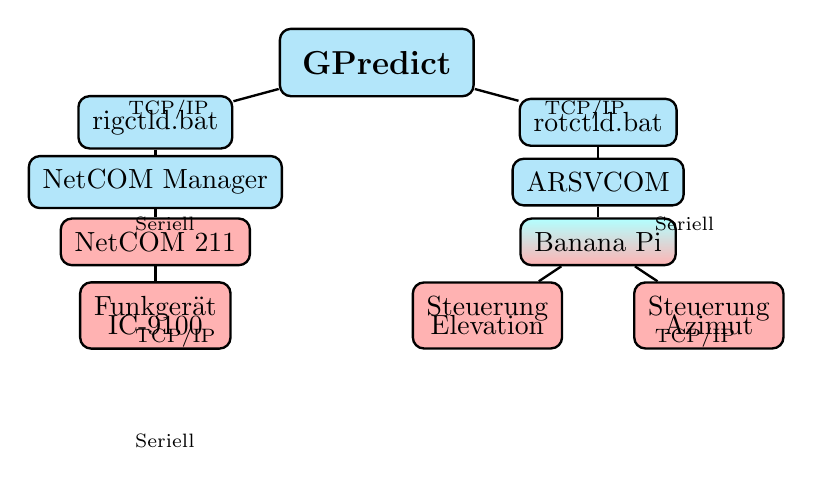
\begin{tikzpicture}[every node/.style = {shape=rectangle, rounded corners, draw, align=center, scale=1}, line width=0.3mm, level distance=1.8\baselineskip, level 1/.style = {sibling distance=16em}, level 2/.style = {sibling distance=8em}]
	\tikzstyle{top} = [fill=cyan!30, inner sep=8pt, font=\bfseries\large]
	\tikzstyle{sw} = [fill=cyan!30, inner sep=5pt]
	\tikzstyle{hw} = [fill=red!30, inner sep=5pt]
	\tikzstyle{hwsw} = [top color=cyan!30, bottom color=red!30, inner sep=5pt]
	\tikzstyle{label} = [draw=none, font=\scriptsize, right]
	\node[top]{GPredict}
	child { node[sw]{rigctld.bat} 
		child { node[sw]{NetCOM Manager} 
				child { node[hw]{NetCOM 211}
					child { node[hw, yshift=-0.5em]{Funkgerät\\[-0.5em]IC-9100} } } } }
	child { node[sw]{rotctld.bat}
		child { node[sw]{ARSVCOM}
			child { node[hwsw]{Banana Pi} 
				child { node[hw, yshift=-0.5em]{Steuerung\\[-0.5em]Elevation} }
				child { node[hw, yshift=-0.5em]{Steuerung\\[-0.5em]Azimut} } } } };
	\node[label] at (2,-0.6) {TCP/IP};
	\node[label,left] at (-2,-0.6) {TCP/IP};
	\node[label] at (-3.2,-2.05) {Seriell};
	\node[label] at (3.4,-2.05) {Seriell};
	\node[label] at (-3.2,-3.5) {TCP/IP};
	\node[label] at (3.4,-3.5) {TCP/IP};
	\node[label] at (-3.2,-4.8) {Seriell};	
\end{tikzpicture}
	\caption{Kommunikation zwischen Hard- und Software}
	\label{fig:swhwcom} 
\end{figure}

Hierbei kommuniziert GPredict über eine IP-basierte Schnittstelle nur mit den HamLib-Programmen \myemph{rigctld.exe} und \myemph{rotctld.exe}. Diese werden unter Berücksichtigung der notwendigen Parameter als Batch-Skripte ausgeführt und müssen solange eine Kommunikation zwischen GPredict und Funkgeräten bzw. Rotoren bestehen soll, aktiv sein.\newpar
Die Software \myemph{NetCOM Manager} stellt eine virtuelle serielle Schnittstelle (COM5) zur Verfügung, auf die von \myemph{rigctl(d).exe} zugegriffen werden kann. Das \myemph{NetCOM 211}-Modul ist wiederum per serieller Schnittstelle mit dem Funkgerät verbunden und ermöglicht die Kommunikation über das Netzwerk mit der Software \myemph{NetCOM Manager}. Somit muss man sich lediglich im Hochschul-Netzwerk befinden, um mit dem Funkgerät kommunizieren zu können. Wird hierbei die Möglichkeit einer VPN-Verbindung wahrgenommen, kann quasi von jedem beliebigen Ort mit Internetanbindung mit dem Funkgerät kommuniziert werden.\newpar
Für die Kommunikation mit den Rotoren, wird auf die Software \myemph{ARSVCOM} zurückgegriffen. Diese emuliert eine Rotorensteuerung vom Typ \myemph{Yaeso RS232A}, wofür ebenfalls ein virtueller, beliebig einstellbarer COM-Port erstellt wird. Der COM-Port und der Rotorensteurungs-Typ werden als Parameter bei \myemph{rotctl(d).exe} angegeben. Die Software \myemph{ARSVCOM} kommuniziert über das Netzwerk mit dem Banana Pi, an welchem wiederum die Steuerungseinheiten des Azimut- und Elevations-Rotors angeschlossen sind (siehe Abschnitt XXX).

\subsection{Test der Bedienfelder}

Um sich mit den Bedienfeldern zur Funkgerät- bzw. Rotorensteuerung vertraut zu machen, kann auf zwei sogenannte \myemph{Dummy}-Schnittstellen zugegriffen werden. Diese sind sowohl bei \myemph{rigctl.exe}, als auch bei \myemph{rotctl.exe} unter der \myemph{Hamlib ID} 1 erreichbar. In Abbildung \ref{fig:dummysettings} ist eine beispielhafte Konfiguration zu sehen, die in den \myemph{Interface}-Einstellungen zur Kommunikation mit den \myemph{Dummy}-Schnittstellen vorgenommen werden kann.

\begin{figure}[h]
	\centering
	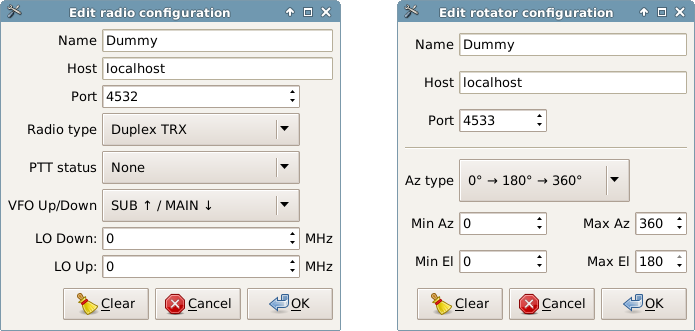
\includegraphics[width=0.6\textwidth]{dummy-settings}
	\caption{Schnittstellenkonfiguration für das Dummy-Interface}
	\label{fig:dummysettings} 
\end{figure}

Für diesen Test wurden für die Programme \myemph{rigctld.exe} und \myemph{rotctld.exe} ebenfalls eigene Batch-Skripte erstellt (siehe Anhang \ref{chap:rigctlddummybat} und \ref{chap:rotctlddummybat}). Die hierfür verwendeten Optionen unterscheiden sich lediglich im Port, für \myemph{rigctld.exe} ist standardmäßig der Port 4532 und für \myemph{rotctld.exe} der Port 4533 vorgesehen. Dieser kann jedoch nach Belieben angepasst werden.
\clearpage
Sobald ein Fehler bei der Kommunikation zwischen den Bedienfeldern und den HamLib-Programmen fünf Mal in Folge aufgetreten ist, wird aus Sicherheitsgründen die Kommunikation automatisch abgebrochen.

\subsection{Test der Kommunikation zum Funkgerät}
\label{chap:rigtest}

Um die Kommunikation zwischen HamLib und dem Funkgerät zu testen, werden zunächst einzelne Kommandos mit Hilfe des Skripts \myemph{rigctl.bat} an das Funkgerät geschickt. Somit kann sichergestellt werden, ob das HamLib-\acl{BE} für das Funkgerät IC-9100 richtig implementiert wurde. Hierbei kann nicht davon ausgegangen werden, dass ein reibungsloser Betrieb möglich ist, da als Test-Status des HamLib-\acl{BE}s für das Funkgerät IC-9100 ,,Untested'' angegeben ist (siehe Seite \pageref{hamlibbackend}).\newpar
In der Betriebsanleitung des Funkgeräts IC-9100 (siehe \cite{radiomanual}) ist auf Seite 183ff eine Übersicht der Befehlsstruktur und der zulässigen Kommandos des ICOM-spezifischen Protokolls CI-V dargestellt. Zur Kontrolle, ob die HamLib-Befehle auch den richtigen CI-V-Kommandos entsprechen, wird mit dem Windows-Programm \myemph{Serial Port Monitor} (hierfür kann auch ein anderes Programm verwendet werden) der serielle Port COM5 abgehört, während über \myemph{rigctl.bat} verschiedene Befehle an das Funkgerät geschickt werden.\newpar
Für die folgenden grundlegenden Befehle konnte eine Übereinstimmung der von HamLib verwendeten mit den in \cite{radiomanual} zu findenden CI-V Befehlen festgestellt und damit eine korrekte Funktionalität sichergestellt werden:

\begin{itemize}
	\parskip0pt
	\item \texttt{F: set\_freq} (Setzen der Frequenz des \myemph{Main}-Bandes)
	\item \texttt{f: get\_freq} (Auslesen der Frequenz des \myemph{Main}-Bandes)
	\item \texttt{M: set\_mode} (Setzen des Modus und der entsprechenden Bandbreite)
	\item \texttt{m: get\_mode} (Auslesen des Modus und der zugehörigen Bandbreite)
\end{itemize}

Eine Übersicht der gültigen Eingabeparameter von \myemph{rigctl(d).exe} kann über die Option \texttt{-\,-dump-caps} ausgegeben werden (siehe Abschnitt \ref{chap:hamlibusage}).

\clearpage

Da das Funkgerät in den meisten Fällen bei der Kommunikation mit Satelliten im Satellitenmodus betrieben werden muss, ist es essentiell, dass dieser über \myemph{rigctl(d).exe} aktiviert werden kann.\label{satmode} Beim Test des entsprechenden Befehls (siehe Tabelle \ref{tab:civcommands}), wurde jedoch festgestellt, dass das CI-V-Kommando, dass an das Funkgerät geschickt wird, nicht dem Korrekten aus \cite{radiomanual} entspricht. Für das fertig kompilierte Programm \myemph{rigctl(d).exe} gibt es zwar den Befehl \texttt{send\_cmd} mit dem laut \cite{hamlibmanual} ASCII-Zeichen geschickt werden können, dieser konnte im Rahmen dieses Projektes jedoch nicht erfolgreich verwendet werden. Es konnte hierbei auch nach Testen verschiedener Teile des CI-V-Kommandos der Satellitenmodus am Funkgerät nicht aktiviert werden. Somit ist es nicht möglich einen ,,rohen'' Befehl zu versenden, ohne einen Eingriff in den Quellcode von HamLib vorzunehmen. In Tabelle \ref{tab:civcommands} ist der HamLib-Befehl zur Aktivierung des Satellitenmodus, das verwendete CI-V-Kommando und das tatsächliche CI-V-Kommando dargestellt. Die Ausschnitte, die nicht übereinstimmen, sind rot markiert.

\begin{table}[h]	 
	\small\begin{tabularx}{\textwidth}{|X|l|l|}
		\hline
		\textbf{HamLib-Befehl \myemph{rigctl(d).exe}}	& \textbf{CI-V (Verwendet)}			&\textbf{CI-V (Tatsächlich)}\\
		\hline
		\texttt{U SATMODE 1}	& \texttt{FE FE 7C E0 \myredtext{1A 07} 01 FD}	& \texttt{FE FE 7C E0 16 5A 01 FD}\\
		\hline		
	\end{tabularx}
	\caption{Fehlerhaftes CI-V Kommando beim Aktivieren des Satellitenmodus}
	\label{tab:civcommands}
\end{table}

\subsection{Test der Kommunikation zu den Rotoren}

Beim Test der Bedienelemente kann der Ausgabe des Skripts \myemph{rotctld-dummy.bat} bei Verwendung der höchsten Ausgabeintensität \texttt{-vvvvv} entnommen werden, dass lediglich die Befehle \texttt{set\_pos} und \texttt{get\_pos} beim Verfolgen eines Satelliten verwendet werden. Diese beiden Befehle konnten mit dem Skript \myemph{rotctl.bat} erfolgreich für die Steuerung der beiden Rotoren getestet werden. Grundsätzlich sind bei der Steuerung der Rotoren einige Aspekte zu beachten, beispielsweise, dass die Rotorgeschwindigkeit reduziert wird, sobald sich der Ist-Winkel in gewisser Nähe zum Soll-Winkel befindet. Diese Punkte werden jedoch alle entweder von den Steuerungsmodulen oder von der Software \myemph{ARSVCOM} übernommen, sodass in GPredict lediglich die jeweiligen Winkel ausgelesen und gesetzt werden müssen.

\clearpage

\subsection{Konfiguration des Funkgeräts}
\label{chap:radioconfig}

Dem Abschnitt XXX kann entnommen werden, dass das Funkgerät IC-9100 vollduplexfähig ist und bei Betrieb im Satellitenmodus nur im \myemph{Sub}-Band senden und im \myemph{Main}-Band empfangen darf. Diese Informationen können in den \myemph{Interface}-Einstellungen wie in Abbildung \ref{fig:radioconfig} zu sehen, eingestellt werden. 

\begin{figure}[h]
	\centering
	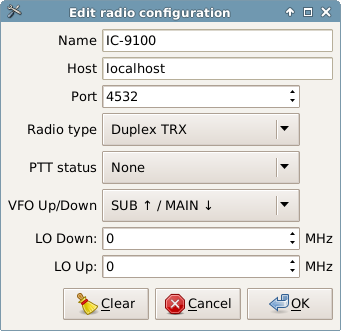
\includegraphics[width=0.3\textwidth]{radiosettings}
	\caption{Funkgerät-Konfiguration}
	\label{fig:radioconfig} 
\end{figure}

Bei \myemph{Host} muss die IP-Adresse angegeben werden unter der aktive \myemph{rigctld.exe}-Prozess zu erreichen ist. Hier ist standardmäßig \myemph{localhost} eingetragen, was für den Computer steht, auf dem GPredict ausgeführt wird. Da im Rahmen dieses Projekts GPredict und \myemph{rigctld.bat} immer auf dem gleichen Computer ausgeführt werden, wird sowohl unter GPredict als auch beim Skript \myemph{rigctld.bat} die IP-Adresse 127.0.0.1 (\myemph{localhost}) eingestellt. Hierbei ist darauf zu achten, dass die Verwendung der Zeichenkette \myemph{localhost} unter Windows bei der Verwendung von \myemph{rigctld.exe} nicht funktioniert. Die Angabe des Ports der \myemph{Interface}-Einstellungen muss ebenfalls dem in \myemph{rigctld.bat} eingestellten Port entsprechen. Die Felder \myemph{LO Down} und \myemph{LO Up} ermöglichen die Berücksichtigung eines Transverters, welcher zur Veränderung der Empfangs- oder Sendefrequenz eingesetzt wird. Somit kann beispielsweise mit einem 28\,MHz-Empfänger ein Signal von einem Satellit der mit 144\,MHz sendet, empfangen werden, in dem 144\,MHz -- 28\,MHz = 116\,MHz bei \myemph{LO Down} eingetragen wird. Beim Feld \myemph{PTT status} wird \myemph{None} eingetragen, da bei vollduplexfähigen Funkgeräten die Abfrage des \ac{PTT}-Status nicht nötig ist (siehe \cite{gpredictmanual} Seite 58).

\clearpage

\subsection{Konfiguration der Rotoren}
\label{chap:rotatorconfig}	

Bei der Konfiguration der Rotorensteuerung ist die Angabe der IP-Adresse und des Ports analog wie bei der Funkgerät-Konfiguration vorzunehmen, bis auf die Ausnahme, dass hier ein anderer Port eingestellt werden muss (siehe Abbildung \ref{fig:rotatorconfig}). 

\begin{figure}[h]
	\centering
	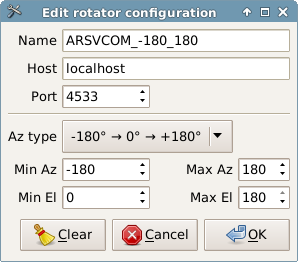
\includegraphics[width=0.25\textwidth]{rotatorsettings180}
	\caption{Mögliche Konfigurationen der Rotorensteuerung}
	\label{fig:rotatorconfig} 
\end{figure}

Der Elevations-Rotor lässt sich von 0\mydegree\ bis 180\mydegree\ auslenken, dementsprechend wird die Einstellung bei \myemph{Min El} und \myemph{Max El} gewählt. Der Azimut-Rotor lässt sich um 360\mydegree\ auslenken und besitzt einen Anschlag bei 180\mydegree\ (Süden), das heißt er lässt sich von 0\mydegree\ (Norden) aus jeweils um 180\mydegree\ in Richtung Süden drehen. Deshalb wird beim Feld \myemph{Az type} der Bereich von -180\mydegree\ bis 180\mydegree\ eingestellt, woraufhin automatisch bei \myemph{Min Az} -180\mydegree\ und bei \myemph{Max Az} 180\mydegree\ eingetragen wird.\newpar
Passiert ein Satellit, wie in Abbildung \ref{fig:rotatorflip} beispielhaft zu sehen, die Linie zwischen dem Mittelpunkt des Polardiagramms und der südlichen Richtung (also den Anschlag des Azimut-Rotors), ist ein Rotorflip notwendig.

\begin{figure}[h]
	\centering
	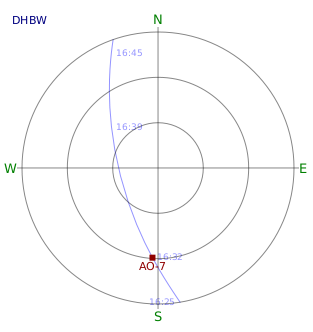
\includegraphics[width=0.35\textwidth]{rotatorflip}
	\caption{Verlauf eines Satelliten über \\den Anschlag des Azimut-Rotors}
	\label{fig:rotatorflip} 
\end{figure}

\newpage

Bei einem Rotorflip wird der Elevations-Rotor über die 90\mydegree-Schwelle gekippt, womit der Anschlag des Azimut-Rotors um 180\mydegree, also nach Norden, verlegt wird. Somit ist es möglich einen Satelliten mit dem in Abbildung \ref{fig:rotatorflip} zu sehenden Verlauf zu verfolgen.

\subsection{Modifizierung des HamLib-Quellcodes}
\label{chap:hamlibmod}

Um fehlerlos einen Rotorflip durchführen zu können, ist es notwendig die Quelldatei, in der das Backend für die verwendete Rotorschnittstelle implementiert ist, anzupassen. Dafür wurden insgesamt drei Änderungen in der Datei \myemph{gs232.c}, die unter dem Pfad \texttt{hamlib-3.0.1/gs232a/} des HamLib-Quellcodes zu finden ist, vorgenommen. Die modifizierte Datei ist im Anhang \ref{chap:hamlibmodification} zu finden.\newpar
Die erste Änderung wurde in der Funktion \texttt{gs232\_rot\_set\_position()} in Zeile 141 vorgenommen. Hier wurde die folgende Zeile eingefügt um sicherzustellen, dass der Azimutwert, der an den Rotor geschickt wird, immer zwischen 0\mydegree\ und 360\mydegree\ liegt:

\vspace{-1em}
\begin{shaded}
	\normalsize{\texttt{if (az < 0.0) az += 360.0;}}
\end{shaded}
\vspace{-1em}

Die zweite Änderung wurde in der Funktion \texttt{gs232\_rot\_get\_position()} in Zeile 171 vorgenommen. Durch Einfügen der folgenden Zeile, wird sichergestellt, dass der vom Rotor gelesene Azimutwert immer zwischen -180\mydegree\ und 180\mydegree\ liegt, sodass er der Rotorkonfiguration von GPredict entspricht:

\vspace{-1em}
\begin{shaded}
	\normalsize{\texttt{if (*az > 180.0) *az -= 360.0;}}
\end{shaded}
\vspace{-1em}

Die dritte Änderung befindet sich in Zeile 224. Hier wurde bei den Fähigkeiten des Rotor-Backends der minimale Azimutwert von 0\mydegree\ auf -180\mydegree\ abgeändert, wie es im Folgenden zu sehen ist:

\vspace{-1em}
\begin{shaded}
	\normalsize{\texttt{.min\_az = -180.0,}}
\end{shaded}
%\vspace{-1em}

\subsection{Kompilieren der modifizierten HamLib für Windows}
\label{chap:winbuild}

Um diese Anpassungen des Quellcodes im Programm \myemph{rotctl(d).exe} nutzen zu können, ist es erforderlich den Quellcode von HamLib nachdem die Änderungen vorgenommen wurden für Windows zu kompilieren. Wie dabei vorgegangen werden muss, ist im Folgenden schrittweise aufgeführt. Hierfür wurde ein Rechner, auf dem Debian 8.5 (64 bit) installiert ist, verwendet.

\begin{enumerate}
	\parskip0pt
	\item Zuerst lädt man den HamLib-Quellcode, der unter \cite{hamlibdownload} verfügbar ist, herunter, entpackt das Archiv \myemph{hamlib-3.0.1.tar.gz} und verschiebt den darin enthaltenen Ordner \myemph{hamlib-3.0.1} ins Verzeichnis \texttt{/home/<username>/builds/}. Das bei Schritt 5 erwähnte Skript bezieht sich auf diesen absoluten Pfad.
	\item Als nächstes lädt man das Archiv \myemph{libusb-win32-bin-1.2.4.0.zip} herunter (siehe \cite{libusbdownload}) und entpackt es ebenfalls in das im vorherigen Schritt genannte Verzeichnis.
	\item Da der Quellcode für die Verwendung unter Windows kompiliert werden soll, müssen unter Linux entsprechende Softwarekomponenten installiert sein. Diese können mit folgenden Befehlen installiert werden:
	\vspace{-1em}
	\begin{shaded}
		\texttt{\$ sudo apt-get update}\\[-0.5em]
		\texttt{\$ sudo apt-get install mingw32 wine}
	\end{shaded}
	\vspace{-1em}	
	\item Nun navigiert man in einer Bash-Kommandozeile in den Ordner \myemph{hamlib-3.0.1} der im ersten Schritt erstellt wurde und führt folgenden Befehl aus:
	\vspace{-1em}
	\begin{shaded}
		\texttt{\$ ./configure --host=i586-mingw32msvc}
	\end{shaded}
	\vspace{-1em}
	\item Anschließend markiert man das Bash-Skript \myemph{build-win32.sh} im Verzeichnis \texttt{./scripts/} mit folgendem Befehl als ausführbar:
	\vspace{-1em}
	\begin{shaded}
		\texttt{\$ chmod +x build-win32.sh}
	\end{shaded}
	\vspace{-1em}	
	\item Als letztes führt man das Bash-Skript \myemph{build-win32.sh} mit folgendem Befehl aus und findet nach erfolgreichem Erstellungsvorgang das Archiv \myemph{hamlib-win32-3.0.1.zip} im Ordner \myemph{hamlib-3.0.1}. In diesem Archiv ist nun die vollständige HamLib für Windows enthalten.
	\vspace{-1em}
	\begin{shaded}
		\texttt{\$ ./build-win32.sh hamlib-3.0.1}
	\end{shaded}
	\vspace{-1em}	
\end{enumerate}

Nähere Details zu den oben genannten Schritten können aus folgenden Dateien des HamLib-Quellcodes (im Ordner \myemph{hamlib-3.0.1}) entnommen werden:

\begin{itemize}
	\parskip0pt
	\item \texttt{INSTALL} (Abschnitt ,,MS Windows'')
	\item \texttt{scripts/README.build-win32} (gesamte Datei)
\end{itemize}

\subsection{Probelauf und Testergebnisse}
\label{chap:probelauf}

Für den korrekten Betrieb von GPredict ist es notwendig folgende Softwarekomponenten zu starten:

\begin{itemize}
	\parskip0pt
	\item Die beiden Skripte \myemph{rigctld.bat} und \myemph{rotctld.bat}
	\item Die Software ARSVCOM
	\item Die Standard-Benutzeroberfläche von GPredict
	\item Die Bedienfelder für die Funkgerät- und Rotorensteuerung
\end{itemize}

Es konnte durch mehrere Probeläufe der grundsätzliche Betrieb von GPredict sichergestellt werden. Dazu gehören das erfolgreiche Ausrichten der Antenne, also des Azimut- und Elevations-Rotors, sowie die Übermittlung der korrekten Frequenz (inklusive Korrektur der Doppler-Verschiebung) zum Funkgerät. Allerdings muss an dieser Stelle auf gewisse Einschränkungen hingewiesen werden, die den reibungslosen Betrieb der Bodenstation mit GPredict noch nicht ganz ermöglichen. Diese sind im Folgenden näher erläutert:\newpar
Möchte man, nachdem die Kommunikation zwischen GPredict und dem Funkgerät erfolgreich aufgebaut ist und diese auch schon eine gewisse Zeit ohne Unterbrechung läuft, von einem Transponder des aktuellen Satelliten auf einen anderen Transponder wechseln, bei dem die \myemph{Down-} und \myemph{Uplink-}Frequenz genau vertauscht sind, bricht die Kommunikation zum Funkgerät ab. Das hat damit zu tun, dass es nicht erlaubt ist, im Satellitenmodus des Funkgeräts die gleiche Frequenz im \myemph{Sub-} und \myemph{Main-}Band einzustellen. Dafür gibt es beim CI-V Protokoll einen speziellen Befehl, der einen Tausch der Frequenzen im \myemph{Sub-} und \myemph{Main-}Band veranlasst. Dieser Befehl wird nicht von dem HamLib-Programm \myemph{rigctld.exe} geschickt. Beim Test unter SatPC32 ist dieser Wechsel möglich und es konnte nachgewiesen werden, dass dort dieser Befehl gesendet wird. Um diese Funktionalität in GPredict zu implementieren, ist ein Eingriff in den Quellcode nötig.\newpar
Wie bereits unter Abschnitt \ref{chap:rigtest} auf Seite \pageref{satmode} beschrieben, ist der Befehl zur Aktivierung des Satellitenmodus des Funkgeräts in HamLib fehlerhaft implementiert. Außerdem wurde festgestellt, dass dieser Befehl beim Kommunikationsaufbau auch nicht vom Skript \myemph{rigctld.bat} an das Funkgerät geschickt wird (bei SatPC32 konnte dies nachgewiesen werden). Somit ist es notwendig, das Funkgerät manuell in den Satellitenmodus zu setzen um eine fehlerfreie Kommunikation zu gewährleisten. Um diese Funktionalität zu gewährleisten, führt ebenfalls kein Weg daran vorbei, den Quellcode von HamLib anzupassen anschließend das Programm \myemph{rigctl.exe} neu zu kompilieren.\newpar
\textbf{Folgenden Abschnitt bzgl. hamlibmodification anpassen!!!}\newpar
Der letzte Punkt, der einem reibungslosen Betrieb von GPredict im Weg steht, hat mit der Konfiguration der Rotorensteuerung zu tun (siehe Abschnitt \ref{chap:rotatorconfig}).\label{rotatorflip2} Hier wurde bereits darauf hingewiesen, dass es bei  entsprechendem Verlauf eines Satelliten notwendig ist, einen Rotorflip durchzuführen. Diesbezüglich konnte nach mehreren Probeläufen mit verschiedenen Satellitenverläufen festgestellt werden, dass die linke Konfiguration auf Abbildung \ref{fig:rotatorconfig} auf Seite \pageref{fig:rotatorconfig} nur dann zu einem fehlerfreien Betrieb führt, wenn der zu verfolgende Satellit den Anschlag des Azimut-Rotors überschreitet (siehe Abbildung \ref{fig:rotatorflip}, Seite \pageref{fig:rotatorflip}). Möchte man mit dieser Konfiguration einen Satelliten verfolgen, der nicht den Anschlag überschreitet, wird dem Azimut-Rotor ein um 180\mydegree\ versetzter Winkel mitgeteilt, was zu einer Fehlpositionierung der Antenne führt. Wählt man die rechte Konfiguration auf Abbildung \ref{fig:rotatorconfig} auf Seite \pageref{fig:rotatorconfig}, so verhält es sich genau umgekehrt, das heißt hiermit ist nur die Verfolgung eine Satelliten möglich, der nicht den Anschlag des Azimut-Rotors passiert. Somit muss vor der Verfolgung eines Satelliten, dessen Verlauf analysiert werden und die entsprechende Konfiguration der Rotorensteuerung ausgewählt werden.\newpar
\textbf{Hardy fragen ob Rotorkonfiguration so passt!!!}\newpar